% Autor: Leonhard Segger, Alexander Neuwirth
% Datum: 2017-10-30
\documentclass[
	% Papierformat
	a4paper,
	% Schriftgröße (beliebige Größen mit „fontsize=Xpt“)
	12pt,
	% Schreibt die Papiergröße korrekt ins Ausgabedokument
	pagesize,
	% Sprache für z.B. Babel
	ngerman
]{scrartcl}

% Achtung: Die Reihenfolge der Pakete kann (leider) wichtig sein!
% Insbesondere sollten (so wie hier) babel, fontenc und inputenc (in dieser
% Reihenfolge) als Erstes und hyperref und cleveref (Reihenfolge auch hier
% beachten) als Letztes geladen werden!

% Silbentrennung etc.; Sprache wird durch Option bei \documentclass festgelegt
\usepackage{babel}
% Verwendung der Zeichentabelle T1 (Sonderzeichen etc.)
\usepackage[T1]{fontenc}
% Legt die Zeichenkodierung der Eingabedatei fest, z.B. UTF-8
\usepackage[utf8]{inputenc}
% Schriftart
\usepackage{lmodern}
% Zusätzliche Sonderzeichen
\usepackage{textcomp}

% Mathepaket (intlimits: Grenzen über/unter Integralzeichen)
\usepackage[intlimits]{amsmath}
% Ermöglicht die Nutzung von \SI{Zahl}{Einheit} u.a.
\usepackage{siunitx}
% Zum flexiblen Einbinden von Grafiken (\includegraphics)
\usepackage{graphicx}
% Abbildungen im Fließtext
\usepackage{wrapfig}
% Abbildungen nebeneinander (subfigure, subtable)
\usepackage{subcaption}
% Funktionen für Anführungszeichen
\usepackage{csquotes}
\MakeOuterQuote{"}
% Zitieren, Bibliographie
\usepackage{biblatex}


% Zur Darstellung von Webadressen
\usepackage{url}
%chemische Formeln
\usepackage[version=4]{mhchem}
% siunitx: Deutsche Ausgabe, Messfehler getrennt mit ± ausgeben
\usepackage{floatrow}
\floatsetup[table]{capposition=top}
\usepackage{float}
% Verlinkt Textstellen im PDF-Dokument
\usepackage[unicode]{hyperref}
% "Schlaue" Referenzen (nach hyperref laden!)
\usepackage{cleveref}
\sisetup{
	locale=DE,
	separate-uncertainty
}
%\bibliography{14Mo_O3_18-06-2018_References}
%TODO anpassen

\begin{document}
	
	\begin{titlepage}
		\centering
		{\scshape\LARGE Versuchsbericht zu \par}
		\vspace{1cm}
		{\scshape\huge O3 - Polarisation \par}
		\vspace{2.5cm}
		{\LARGE Gruppe 14Mo \par}
		\vspace{0.5cm}
		
		{\large Alexander Neuwirth (E-Mail: a\_neuw01@wwu.de) \par}
		{\large Leonhard Segger (E-Mail: l\_segg03@uni-muenster.de) \par}
		\vfill
		
		durchgeführt am 18.06.2018\par
		betreut von\par
		{\large Kristina Mühlenstrodt}
		
		\vfill
		
		{\large \today\par}
	\end{titlepage}
	\tableofcontents
	\newpage

	%TODO mehr TODO in Default	

	\section{Kurzfassung}
	%TODO Hypothese	und deren Ergebnis, wenn Hypothese ist, dass nur Theorie erfüllt, sagen: Erwartung: Theorie aus einführung (mit reflink) erfüllt
	%TODO Ergebnisse, auch Zahlen, mindestens wenn's halbwegs Sinn ergibt
	%TODO Was wurde gemacht
	%TODO manche leute wollen Passiv oder "man", manche nicht
	
	\section{Methoden}
	%TODO Bilder von der Website klauen
	%TODO einer will Präsens
	
	\section{Ergebnisse und Diskussion}
	%TODO Unsicherheiten
	

	\subsection{Beobachtung und Datenanalyse}
	%TODO Einflüsse von veränderten Parametern auf Messung
	\subsubsection{Unsicherheiten} %TODO GGF IN DATENANYLSY
	Die Unsicherheiten werden gemäß GUM ermittelt. 
	Außerdem wird für Unsicherheitsrechnungen die Python Bibliothek "uncertainties" verwendet.
	\begin{description}
		\item[Photodiode/Multimeter:] Der Messwert der Photodiode wird auf einem Multimeter abgelesen. 
			Das Multimeter zeigt die Spannung mit 3 Nachkommastellen an. 
			Es würde sich also eine Unsicherheit von \SI{0,0003}{V} ergeben (rechteckige WDF). %TODO wieso Konjunktiv?
			Bei allen Messungen außer dem Überprüfen des Gesetz von Malus und der Untersuchung der $\lambda/2$-Platte müsste die Photodiode nach jedem Verändern der Systemparameter rejustiert werden, damit der Laserstrahl wieder mittig auf die Photodiode trifft. 
			Daher wird für diese Messungen die Unsicherheit mit \SI{0,003}{V} abgeschätzt. %TODO unsihcherheit ggf höher
		\item[Winkelmessung:]  Die Winkel werden mit dem Auge anhand einer Skala abgelesen, wobei die Unsicherheit für den Polarisator/Analysator und die $\lambda/2$-Platte \SI{0,4}{\degree} beträgt. 
			Beim Einstellen des Analysatorwinkels bei der Bestimmung der Konzentration der Zuckerlösung ändert sich die gemessene Intensität des transmitierten Strahls kaum in Abhängigkeit von dem Winkel nahe dem Maximum. 
			Insofern wird eine Unsicherheit von \SI{2}{\degree} angenommen.
			Die Skala des Winkelmessarmes ist kleiner als die der Polarisatoren und der Arm hat beim Konfigurieren etwas Spielraum. 
			Folglich wägen wir die Unsicherheit mit \SI{0,8}{\degree} ab.
	\end{description} 

	\subsubsection{Gesetz von Malus}
	Das Multimeter, das an die Photodiode angeschlossen ist, zeigt eine Spannung von \SI{0,060+-0,001}{V} an, während der Laser ausgeschaltet war.
	Beim Vergleichen der Intensitäten mit nur einem Polarisator zeigt sich, dass der Laser einen höheren p-polarisierten als s-polarisierten Anteil erzeugt.
	In \cref{fig_Malus1} ist die Lichtintensität gegen den Analysatorwinkel $\alpha$ relativ zum Polarisator aufgetragen.
	Der Analysatorwinkel wird in \SI{10}{\degree}-Schritten von \SI{-90}{\degree} bis \SI{90}{\degree} variiert.

	\begin{figure}[H] %TODO cos^2 reinfitten?
		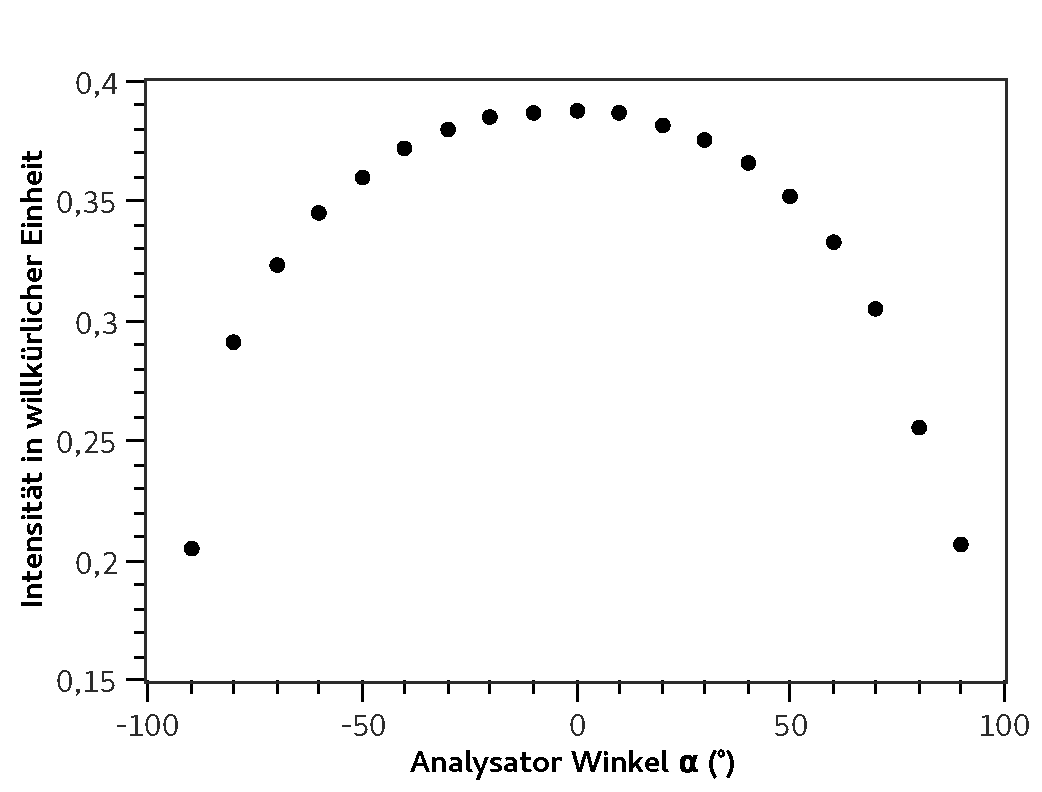
\includegraphics[width=0.7\textwidth]{fig_Malus1}
		\centering
		\caption{Ein Laserstrahl wird zuerst durch einen Polarisator und dann durch einen Analysator gelenkt. 
		Der Winkel zwischen Polarisator und Analysator ist auf der X-Achse dargestellt. 
		Hinter dem Analysator wird mit einer Photodiode und eine Multimeter die Intensität gemessen. 
		Diese ist in willkürlichen Einheiten dargestellt. 
		Die Unsicherheiten sind kleiner als die Symbolgröße.} 
		\label{fig_Malus1}
		\centering
	\end{figure}
	\subsubsection{$\lambda/2$-Platte}
	Die $\lambda/2$-Platte wird in \SI{45}{\degree}-Stellung zwischen Polarisator und Analysator positioniert.  
	Der Winkel des Analysators wird so gewählt, dass die Photodiode einen maximale Intensität misst.
	Für die eingestellten \SI{45+-0,4}{\degree} Winkeldifferenz folgt ein Analysatorwinkel von \SI{89+-0,4}{\degree}.
	In \cref{fig_lambda} sind gegen einige anderen Stellungen der $\lambda/2$-Platte die resultierenden Analysatorwinkel aufgetragen. 
	In der Einführung wurde für einen Laserstrahl bei der Trasmission durch eine $\lambda/2$-Platte eine Drehung der Polarisationsebene um $\Delta\beta=2\alpha$, wobei $\alpha$ der Winkel der Platte ist, beschrieben.
	Um dies überprüfen zu können, wurde ein linearer Fit durchgeführt.
	Die Steigung $a=\SI{1,88+-0,06}{}$ gibt den Faktor zwischen $\Delta\beta$ und $\alpha$ an.

	\begin{figure}[H]
		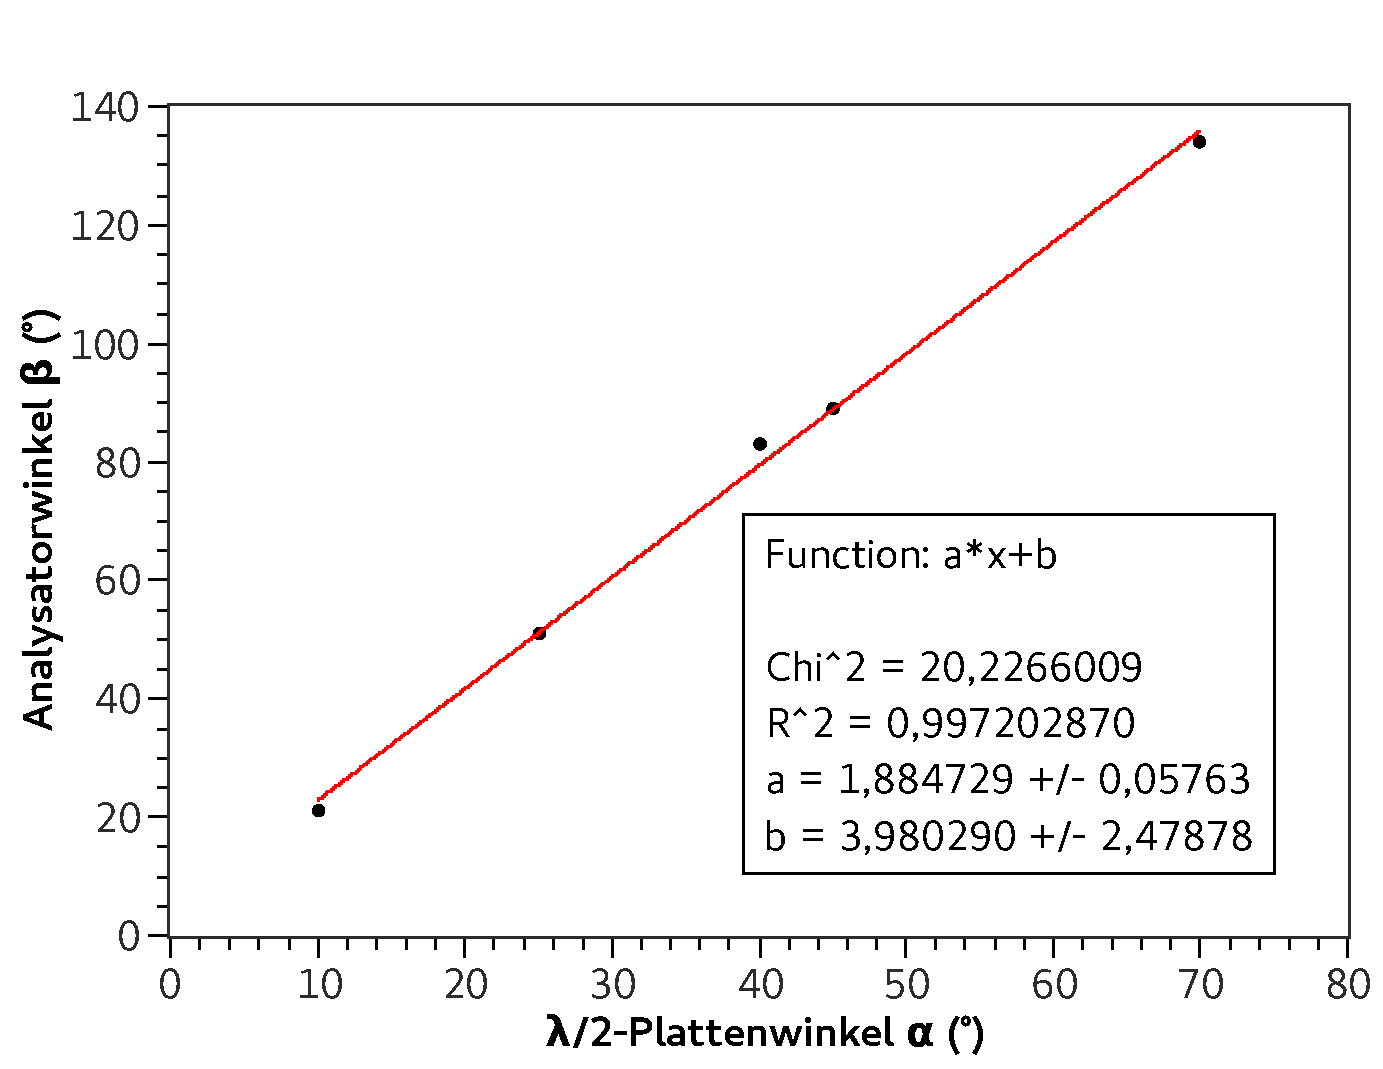
\includegraphics[width=0.7\textwidth]{fig_lambda}
		\centering
		\caption{Ein Laser strahlt als erstes durch einen Polarisator. 
		Darauf folgt eine $\lambda/2$-Platte, die mit einem Winkel $\alpha$ relativ zur Polarisation des eintreffend Strahls ausgerichtet wurde. 
		Vor der Photodiode befindet sich ein Analysator, der so justiert wurde, dass die gemessene Intensität maximal wird.
		Der Winkel $\beta$ des Analysators relativ zum Polarisator wird gegen den Plattenwinkel $\alpha$ aufgetragen.
		Es wird ein linearer Fit durchgeführt.
		Die Unsicherheiten sind kleiner als die Symbole.} %TODO Symbole oder Symbolgröße?
		\label{fig_lambda}
		\centering
	\end{figure}
	\subsubsection{Reflexionsvermögen}
	Es wird ein p bzw. s polarisierter Laserstrahl auf eine Glasplatte mit einem Einfallswinkel $\alpha$ gerichtet.
	In gleichem (Reflexions-)Winkel $\alpha$ wird die Photodiode positioniert.
	Zunächst wird mittels des Analysators vor der Photodiode überprüft, ob sich die Polarisationsrichtung geändert hat. 
	Die Spannung am Multimeter ändert sich nahezu nicht wenn die Polarisationsrichtung gleich der des einfallenden Strahls ist. 
	Ebenso wird die gemessene Intensität minimal für eine Winkeldifferenz von $\SI{\pm90}{\degree}$.
	In \cref{fig_pol} ist die Lichtintensität des reflektierten Lichts gegen den Einfallswinkel $\alpha$ von \SI{30}{\degree} bis \SI{85}{\degree} in \SI{5}{\degree}-Schritten aufgetragen.
	Dabei tritt das Problem auf, dass zwischen jeder Messung die Photodiode so rejustiert werden muss, dass der Laserstrahl diese zentriert trifft.
	Es ist ein deutliches Minimum für die Reflexion von p-polarisiertem Licht erkennbar.
	Laut der Einführung wird im Brewsterwinkel $\alpha_B$ kein p-polarisiertes Licht reflektiert.
	Folglich beträgt der Brewsterwinkel ca. $\alpha_B = \SI{55+-1}{\degree}$.
	Außerdem ist \cref{eq_brech} zur Bestimmung des Brechungsindex gegeben.
	\begin{equation}
		n= \tan(\alpha_B)
		\label{eq_brech}
	\end{equation}
	\begin{equation}
		u(n) = \frac{1}{\cos(\alpha_B)^2} \cdot u(\alpha_B)
		\label{eq_unsicher}
	\end{equation}
	Es ergibt sich ein Brechungsindex $n = \SI{1,43 +- 0,05}{}$
	\footnote{Beim Einsetzten der Werte in \cref{eq_unsicher} ergibt sich eine zu hohe Unsicherheit. Die Python Bibliothek "uncertainties" berechnet einen geringeren Wert, der sich deckt mit direkt in die \cref{eq_brech} eingesetzten Grenzen. Grund hierfür ist wahrscheinlich ein Fehler durch Terme höherer Ordnung.}.

	\begin{figure}[H]
		\centering
		\begin{subfigure}[t]{0.5\textwidth}
			\centering
			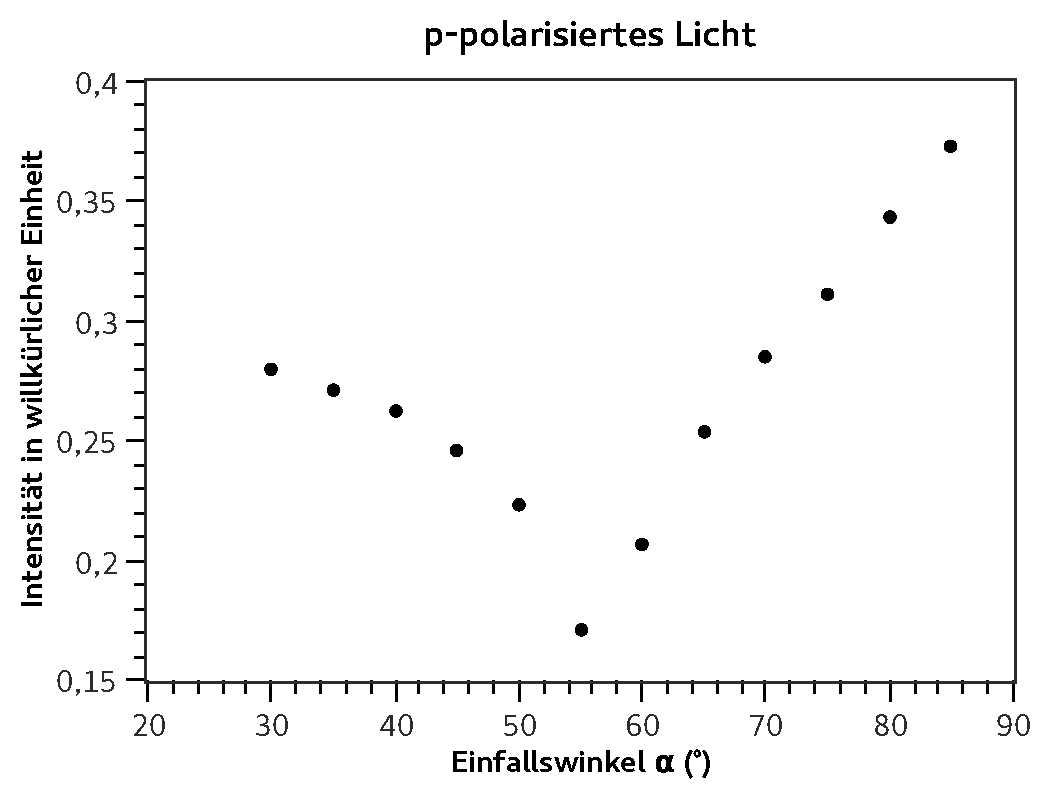
\includegraphics[width=1\textwidth]{fig_ppol}
			\label{fig_ppol}
			\caption{p-polarisiertes Licht}
		\end{subfigure}%
		\begin{subfigure}[t]{0.5\textwidth}
			\centering
			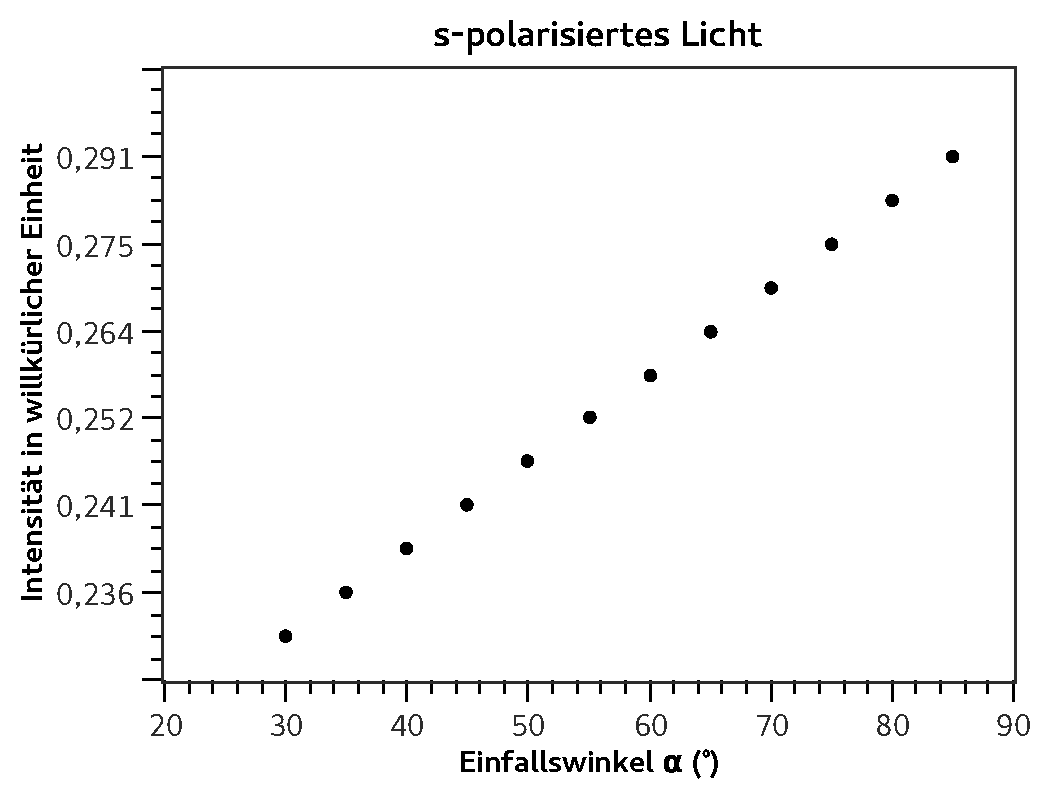
\includegraphics[width=1\textwidth]{fig_spol}
			\label{fig_spol}
			\caption{s-polarisiertes Licht}
		\end{subfigure}
		\label{fig_pol}
		\caption{Ein Laserstrahl wird nach einem Polarisator an einem Glas unter dem Winkel $\alpha$ reflektiert und die Intensität des reflektierten Lichts wird gemessen. 
		Es wurde p und s-polarisiertes Licht untersucht.
		Die Unsicherheiten sind kleiner als die Symbole.}

	\end{figure}


	\subsubsection{Zuckerkonzentration}
	\subsubsection{Kalkspatkristall}
	
	\subsection{Diskussion}
	%TODO Bezug/Nutzen oder sonst was
	%TODO auch hier die Hypothese wiederholen
	%TODO keine Messwerte hier, nach manchen Menschen, zumindest "direkt" erstellte Diagramme net hier, auch wenn Lesbarkeit-bla
	
	%TODO Malus-Kurve-Diskussion: Sättigung der Diode (=> peak ist weniger spitz?!?) und Filter sind nicht exakt (=> Filter Null /= Real Null)
	%TODO Malus-Kurven-Diskussion: Real Null /= Null, von Umgebungslicht und thermische Diodeneffekte
	%TODO Malus-Kurve: (minimale) Asymetrie durch mögliche Verunreinigung des Systems.

	%TODO lambda/2: lambda nicht exakt gleich => offset
	\section{Schlussfolgerung}
	%TODO Rückgriff auf Hypothese und drittes Nennen dieser
	
	%TODO Quellen zitieren, Websiten mit Zugriffsdatum
	%TODO Verweise auf das Laborbuch (sind erlaubt)
	%TODO Tabelle + Bilder mit Beschriftung
	%\printbibliography
\end{document}
